\documentclass{beamer}
\usepackage[latin1]{inputenc}
\usepackage{graphicx}
\usetheme{Antibes}
\usecolortheme{albatross}

\title{The Crank-Nicolson Algorithm in SAGE}
\author{Cody Horst}\institute{University of Washington}

\begin{document}

\begin{frame}
\titlepage

\end{frame}

\begin{frame}
The Reaction-Diffusion equation in one dimension:
\newline
$$\frac{du}{dt} = D\frac{d^{2}u}{dx^{2}} + R(x) $$\\


Numerous applications in finance, pattern formation, chemical kinetics
    
\end{frame}

\begin{frame}
the Crank-Nicolson Algorithm, a classic finite-difference method

\begin{itemize}
  \item these methods approximate derivatives using differences, as the name suggests. This is similar to the definition of a derivative
  \item implicit, guaranteed stable, but not necessarily numerically accurate
\end{itemize}

I wrote a sage class that implements this algorithm, along with convenient plotting functionality built-in.

\end{frame}

\begin{frame}
Crank-Nicolson Implementation: discretization \newline
$
u(x,t) = \frac{u_{i,n+1} u_{i,n+1}}{2}
\newline
\frac{du}{dt} = \frac{u_{i,n+1} - u_{in}}{k}
\newline
\frac{du}{dx} = \frac{u_{i+1,n} - u_{i-1,n}}{h}
\newline
\frac{d^{2}u}{dx^{2}} = \frac{(u_{i+1,n} - 2*u_{i,n} + u_{i-1,n+1}) + (u_{i+1,n+1} - 2*u_{i,n+1} + u_{i-1,n+1})}{2h^{2}}
$ \\

For this I used symbolic math in SAGE
\end{frame}

\begin{frame}
After discretization, the PDE can be arranged into a tri-diagonal matrix as below, which can be solved by LU-decomposition. \newline
$$
\begin{bmatrix}
   {b_1} &  {c_1} & {   } & {   } & { 0 } \\
   {a_2} &  {b_2} & {c_2} & {   } & {   } \\
   {   } &  {a_3} & {b_3} & \ddots & {   } \\
   {   } &  {   } & \ddots & \ddots & {c_{n-1}}\\
   { 0 } &  {   } & {   } & {a_n} & {b_n}\\
\end{bmatrix}
\begin{bmatrix}
   {x_1 }  \\
   {x_2 }  \\
   {x_3 }  \\
   \vdots   \\
   {x_n }  \\
\end{bmatrix}
=
\begin{bmatrix}
   {d_1 }  \\
   {d_2 }  \\
   {d_3 }  \\
   \vdots   \\
   {d_n }  \\
\end{bmatrix}
$$

The Dirichlet boundary condition as the starting point for my implementation.
\end{frame}

\begin{frame}
    $$
    \frac{du}{dt} = D\frac{du^{2}}{dx^{2}}
    $$
    \newline
    x-axis is time, y-axis is spatial
    \newline
    IC: constant
    \newline
  \begin{columns}[T]
    \begin{column}{.5\textwidth}
   
    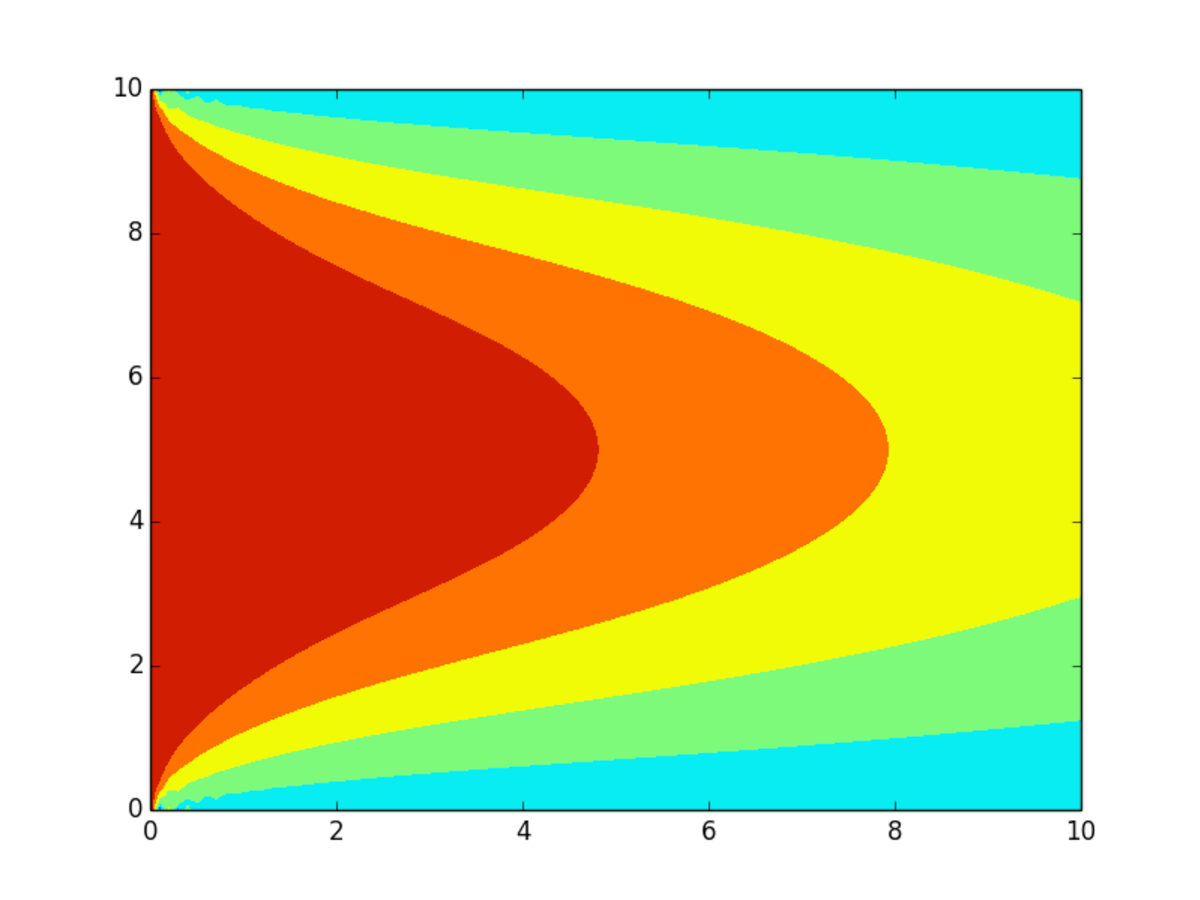
\includegraphics[scale=0.25]{hm1.pdf}
    
    \end{column}
    
    \begin{column}{.5\textwidth}
   
    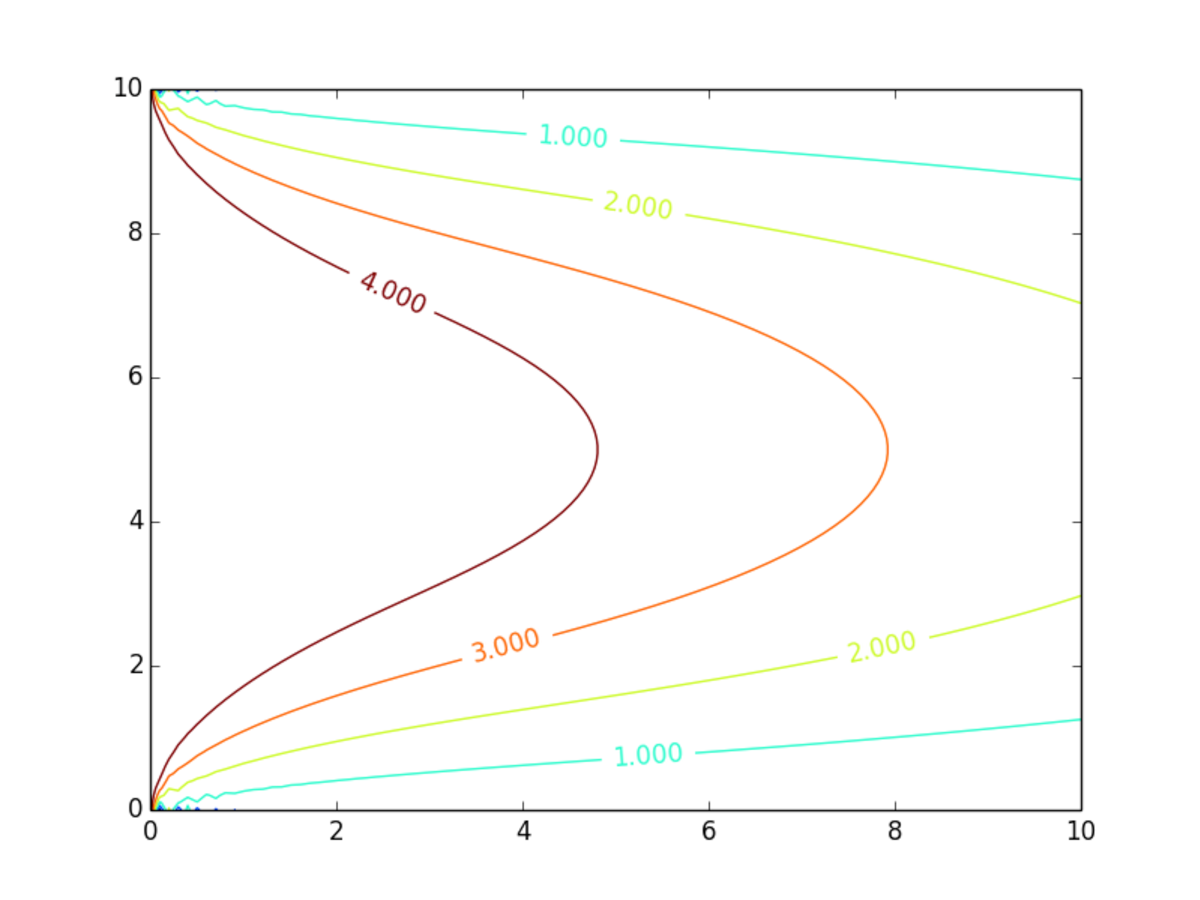
\includegraphics[scale=0.25]{cm1.pdf}
  
    \end{column}
  \end{columns}
\end{frame}

\begin{frame}
     $$
    \frac{du}{dt} = 0.07\frac{du^{2}}{dx^{2}} + 0.5u
    $$
    \newline
    x-axis is time, y-axis is spatial
    \newline
    IC: linear increase
    \newline
    
  \begin{columns}[T]
    \begin{column}{.5\textwidth}
   
    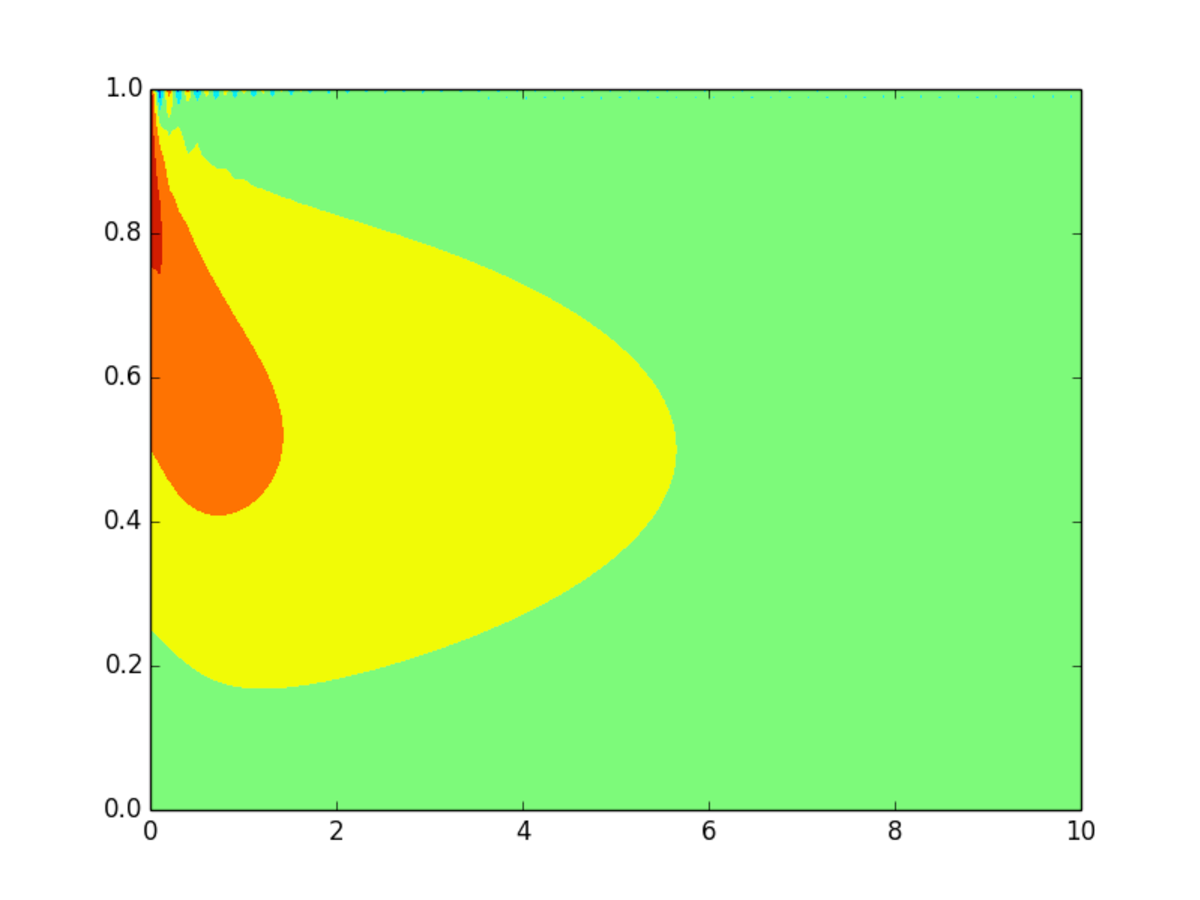
\includegraphics[scale=0.25]{hm2.pdf}
    
    \end{column}
    
    \begin{column}{.5\textwidth}
   
    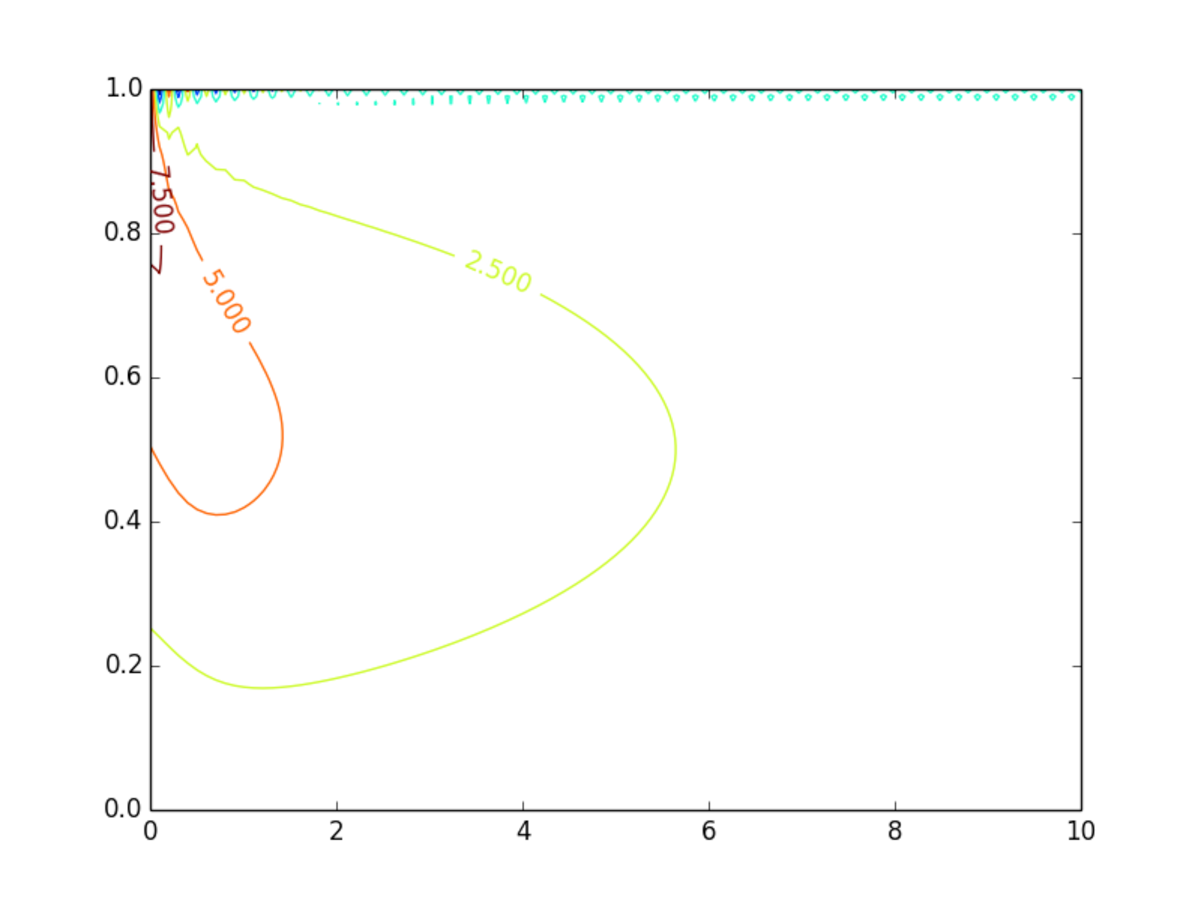
\includegraphics[scale=0.25]{cm2.pdf}
  
    \end{column}
  \end{columns}
\end{frame}

\begin{frame}
    $$
    \frac{du}{dt} = 0.01\frac{du^{2}}{dx^{2}} - 0.07u
    $$
    \newline
    x-axis is time, y-axis is spatial
    \newline
    IC: constant
    \newline
    
  \begin{columns}[T]
    \begin{column}{.5\textwidth}
    
    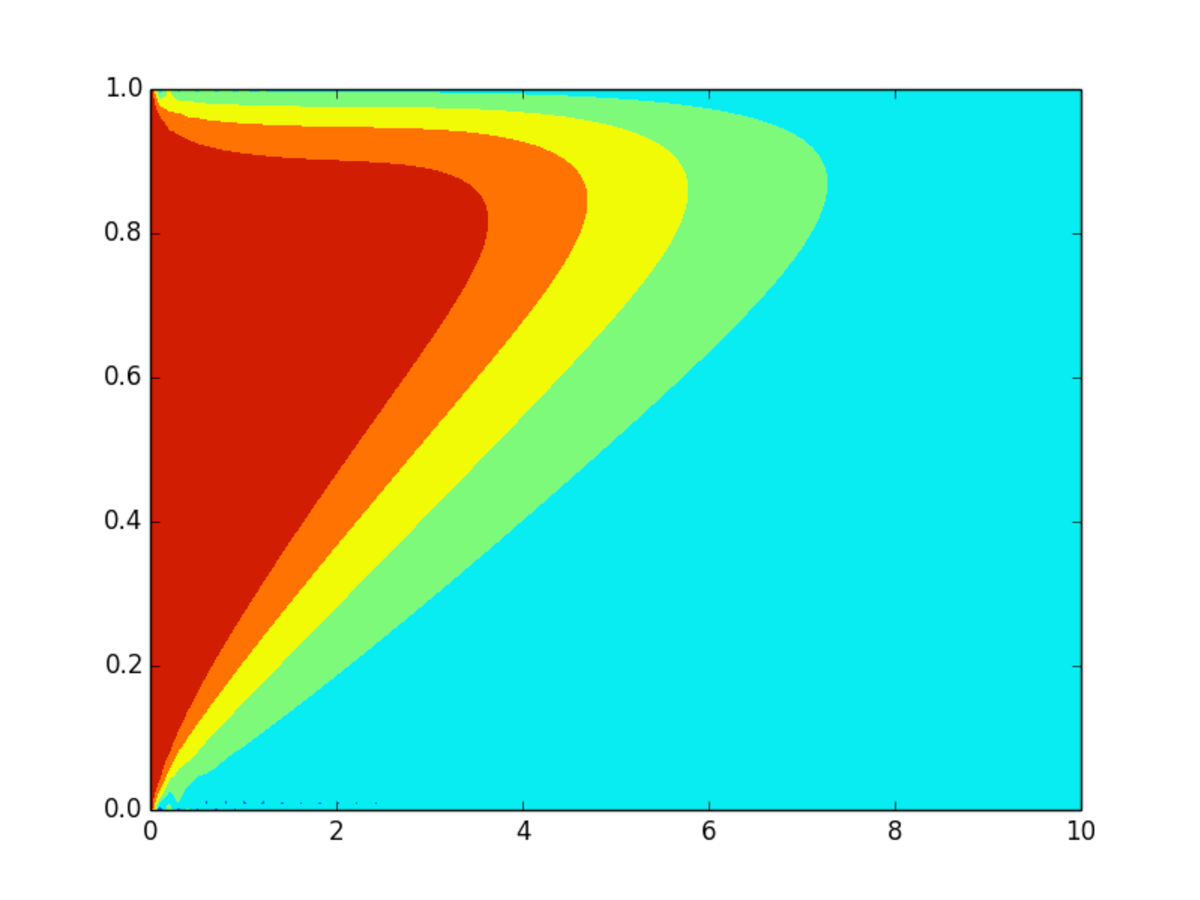
\includegraphics[scale=0.25]{hm3.pdf}
    
    \end{column}
    
    \begin{column}{.5\textwidth}
   
    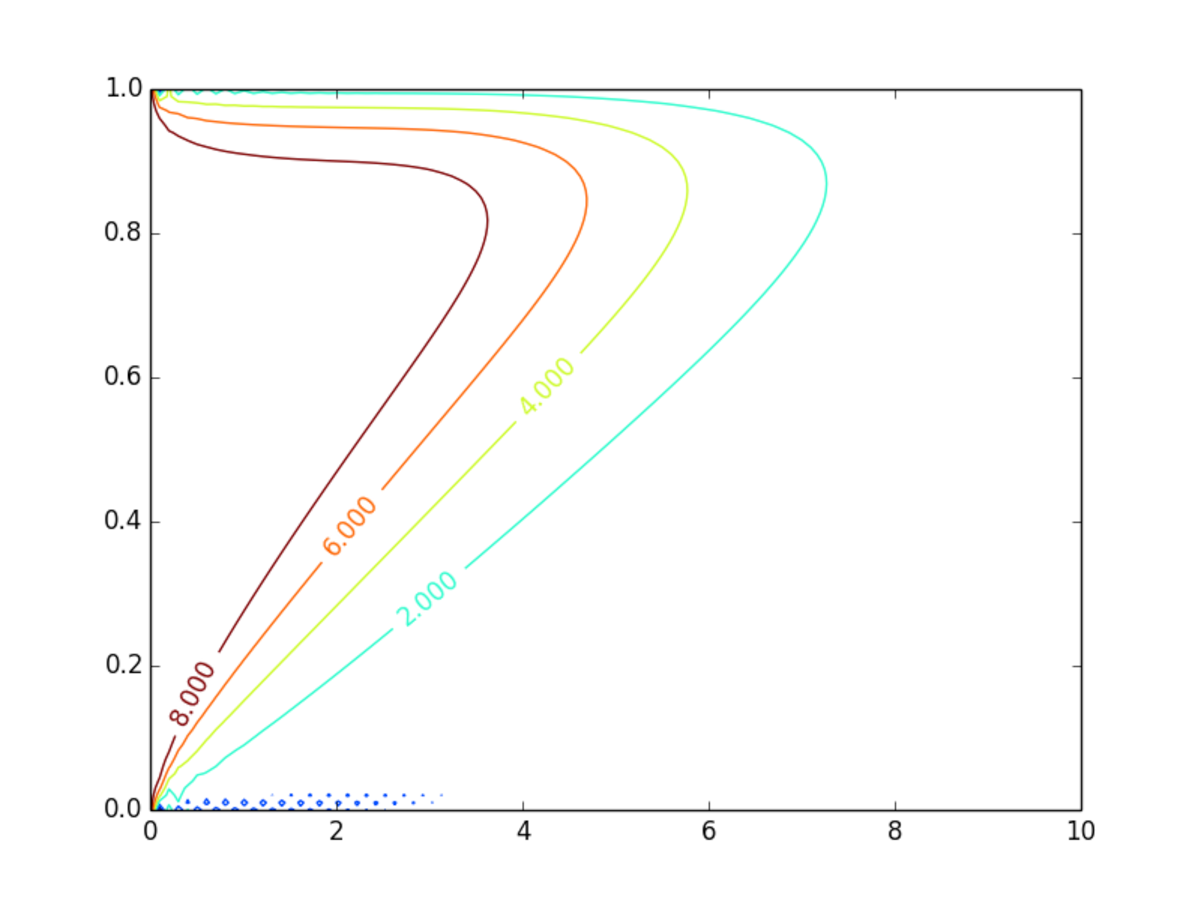
\includegraphics[scale=0.25]{cm3.pdf}
  
    \end{column}
  \end{columns}
\end{frame}

\end{document}
%sagemathcloud={"zoom_width":55}